\documentclass{amsart}
\usepackage[utf8]{inputenc}
\usepackage{enumitem}
\usepackage{physics}
\usepackage{bm}
\usepackage{bbm}
\usepackage{hyperref}
\usepackage{tikz} 
\usetikzlibrary{positioning, arrows, matrix, intersections}
\usepackage{tabularx}
\newcolumntype{C}{>{\centering\arraybackslash}X}
\usepackage{xfrac}
\usepackage{adjustbox}
\usepackage{mathpartir}
\usepackage{quiver}
\usepackage{multicol}
\usepackage{amsmath}
\usepackage{pifont}
\newcommand{\cmark}{\ding{51}}%
\newcommand{\xmark}{\ding{55}}

\tikzset{snake it/.style={decorate, decoration=snake}}

\usepackage{minted}
\usemintedstyle{tango}

\theoremstyle{definition}
\newtheorem{eg}{Example}[section]
\newtheorem{ex}{Exercise}[section]
\newtheorem{defn}{Definition}[section]
\newtheorem*{sol}{Solution}
\newtheorem*{warn}{Warning}
\newtheorem*{fact}{Fact}
\newtheorem*{cor}{Corollary}

\usepackage{pgfplots}
\pgfplotsset{compat=1.12}
\usepgfplotslibrary{fillbetween}

\title[Introduction to HoTT Notes]{OPLSS 2023 \\
Introduction to HoTT Notes}
\author{Pavel Kovalev, Sean O'Connor, Cassia Torczon, Frank Tsai}
\date{July 2023}


\newcommand{\N}{\mathbbm{N}}
\newcommand{\Z}{\mathbbm{Z}}
\newcommand{\Q}{\mathbbm{Q}}
\newcommand{\R}{\mathbbm{R}}
\newcommand{\ctx}{\ensuremath{\mathsf{~ctx}}}
\newcommand{\type}{\ensuremath{\mathsf{~type}}}
\newcommand{\defeq}{\ensuremath{\overset{\boldsymbol{\cdot}}{=}}}
\newcommand{\Unit}{\ensuremath{\mathbbm{1}}}
\newcommand{\Bool}{\ensuremath{\mathsf{Bool}}}
\newcommand{\Prop}{\ensuremath{\mathsf{Prop}}}
\newcommand{\isProp}{\ensuremath{\mathsf{isProp}}}
\newcommand{\Set}{\ensuremath{\mathsf{Set}}}
\newcommand{\isSet}{\ensuremath{\mathsf{isSet}}}
\newcommand{\Cat}{\ensuremath{\mathsf{Cat}}}
\newcommand{\isContr}{\ensuremath{\mathsf{isContr}}}
\newcommand{\isGroupoid}{\ensuremath{\mathsf{isGroupoid}}}
\newcommand{\Rezk}{\ensuremath{\mathsf{Rezk}}}
\newcommand{\isofhlevel}[2]{\ensuremath{\mathsf{isofhlevel}~#1~#2}}
\newcommand{\isEquiv}{\ensuremath{\mathsf{isEquiv}}}
\newcommand{\idToEquiv}{\ensuremath{\mathsf{idToEquiv}}}
\newcommand{\idToIso}{\ensuremath{\mathsf{idToIso}}}
\newcommand{\Iso}{\ensuremath{\mathsf{Iso}}}
\newcommand{\Grp}{\ensuremath{\mathsf{Grp}}}
\newcommand{\Grpd}{\ensuremath{\mathsf{Grpd}}}
\newcommand{\W}{\ensuremath{\mathsf{W}}}
\newcommand{\U}{\ensuremath{\mathcal{U}}}
\newcommand{\True}{\ensuremath{\mathsf{true}}}
\newcommand{\False}{\ensuremath{\mathsf{false}}}
\newcommand{\Ind}{\ensuremath{\mathsf{ind}}}
\newcommand{\Hole}[1]{\fbox{?#1}}
\newcommand{\ob}[1]{\ensuremath{\mathrm{ob}{(\cat{#1})}}}
\newcommand{\cHom}[2]{\ensuremath{\mathrm{Hom}(#1,#2)}}
\newcommand{\cId}{\ensuremath{\mathbf{1}}}
\newcommand{\ua}{\ensuremath{\mathsf{ua}}}
\newcommand{\cat}[1]{\ensuremath{\mathbf{#1}}}
\renewcommand{\emph}{\textbf}
\renewcommand{\emptyset}{\varnothing}

\newcommand{\newcommenter}[3]{%
  \newcommand{#1}[1]{%
    \textcolor{#2}{\small\textsf{[{#3}: {##1}]}}%
  }%
}
\newcommenter{\FT}{red}{FT}

\usepackage[normalem]{ulem}
\newcommand{\surprising}{\textcolor{blue}{s\uwave{urprisin}g} $\text{}$}

\begin{document}

\maketitle
\tableofcontents

\section{Introduction}
\label{sec:introduction}

The fields of Type theory, Set theory, Topos theory, Category theory, Homotopy theory, and Functional programming all matured in the 20th century as their own distinct and influential fields of study. But near the beginning of the 21st century, more and more of the connections across these fields were recognized, which years later culminated in the field of Homotopy Type Theory (HoTT).

\begin{figure}[h]
    \centering
    \[\begin{tikzcd}
	{\text{Type theory}} & {\text{Logic}} & {\text{Set theory}} \\
	{\text{Functional programming}} & {\text{HoTT}} & {\text{Topos theory}} \\
	{\text{Homotopy theory}} && {\text{Category theory}}
	\arrow[no head, from=3-1, to=2-2]
	\arrow[no head, from=2-1, to=2-2]
	\arrow[no head, from=1-1, to=2-2]
	\arrow[no head, from=1-2, to=2-2]
	\arrow[no head, from=1-3, to=2-2]
	\arrow[no head, from=2-3, to=2-2]
	\arrow[no head, from=3-3, to=2-2]
	\arrow[no head, from=1-1, to=1-2]
	\arrow[no head, from=1-2, to=1-3]
	\arrow[no head, from=1-3, to=2-3]
	\arrow[no head, from=2-3, to=3-3]
	\arrow[no head, from=3-3, to=3-1]
	\arrow[no head, from=1-1, to=2-1]
	\arrow[color={rgb,255:red,0;green,0;blue,255}, shorten <=0pt, squiggly, no head, from=3-1, to=2-1]
\end{tikzcd}\]
    \caption{Connections across different fields of mathematics and computer science.
    The blue squiggly line is the surprising connection between homotopy theory and functional programming.}
    \label{fig:connections-across-fields}
\end{figure}

HoTT has strong ties to each of these other fields, and provides a fertile ground for investigating and proving \surprising connections between each of them. This lecture series will provide an introduction to this growing field and will help illuminate its relation to these other areas of study.
HoTT is built on top of Martin-L\"{o}f Type Theory (MLTT), which we introduce in \S\ref{sec:martin-lof-type-theory}.


\section{Martin-L\"{o}f Type Theory}
\label{sec:martin-lof-type-theory}
MLTT consists of 3 basic judgments.
An in-depth treatment of judgments can be found in \cite{ml:justif-log}.
The first judgment expresses that $\Gamma$ is a valid context.
\[
\Gamma \ctx
\]
The second judgment expresses that $\tau$ is a type under the context $\Gamma$, presupposing that $\Gamma \ctx$.
\[
\Gamma \vdash \tau \type
\]
Finally, the last judgment expresses that $t$ is an element of type $\tau$ under the context $\Gamma$, presupposing that $\Gamma \ctx$ and that $\Gamma \vdash \tau \type$.
\[
\Gamma \vdash t : \tau
\]
These three judgments have their corresponding equality judgments.
The first judgment expresses that two valid contexts, $\Gamma$ and $\Gamma'$, are definitionally equal.
\[
\Gamma \defeq \Gamma' \ctx
\]
The second judgment expresses that two types are definitionally equal under the same context $\Gamma$.
\[
\Gamma \vdash \tau \defeq \tau' \type
\]
And the last judgment expresses that two terms, $t$ and $t'$, of type $\tau$ under the context $\Gamma$ are definitionally equal.
\[
\Gamma \vdash t \defeq t' : \tau
\]
\begin{eg}[Some example types in MLTT]
\hfill
\begin{multicols}{2}
\begin{enumerate}
\item Empty type $\varnothing$.
\item Unit type $\Unit$.
\item The type of Boolean $\Bool$.
\item The type of natural numbers $\N$.
\item The types of equalities $=$.
\item Dependent product types $\Sigma$.
\item Dependent function types $\Pi$.
\item Universes $\U_{i}$.
\end{enumerate}
\end{multicols}
\vspace{-\baselineskip}
\begin{enumerate}
    \item[(5)] The types of well-founded trees $\W$. 
\end{enumerate}
\end{eg}

MLTT can be extended with additional features.
Two possible extensions are summarized in Table \ref{tb:extensions-of-mltt}.
\begin{table}[h]
    \centering
    \begin{tabular}{|c||c|c|}\hline
        Type Theory & Univalence Axiom & Higher Inductive Types\\\hline
        UTT  & \cmark & \xmark\\\hline
        HoTT & \cmark & \cmark\\\hline
    \end{tabular}
    \caption{Univalent Type Theory (UTT) is MLTT extended with the Univalence Axiom, and HoTT is UTT extended with higher inductive types.}
    \label{tb:extensions-of-mltt}
\end{table}

\subsection{Inductive Types}
\label{sec:inductive-types}
An inductive type is freely generated by its canonical elements.
To define an inductive type in Coq, one can write
\begin{figure}[H]
    \centering
    \begin{minted}{coq}
        Inductive T : Type := foo : T | bar : T.
    \end{minted}
\end{figure}
The type \texttt{T} is freely generated by its two canonical elements, namely \texttt{foo} and \texttt{bar}.
Coq generates an elimination rule for \texttt{T} automatically.

In general, to specify a new type in type theory we specify:
\begin{enumerate}
    \item how to form new types of this kind via \emph{formation rules}.
    For example, if $A$ and $B$ are types then $A \to B$ is a type.
    \item how to construct canonical elements of that type via \emph{introduction rules}.
    For example, a function type has one introduction rule, namely $\lambda$-abstraction.
    \item how to use elements of that type via \emph{elimination rules}.
    For example, a function type has one elimination rule, namely function application.
    \item how elimination rules act on introduction rules.
    For example, applying a $\lambda$-abstraction $(\lambda x.e)$ to a term $e'$ is definitionally equal to substituting $e'$ for $x$ in $e$, namely $e[\sfrac{e'}{x}]$. 
\end{enumerate}
See the HoTT book \cite{hottbook}.

\subsection{The Booleans}
\label{sec:the-booleans}

The type of Booleans is introduced using formation, introduction, elimination, and computation rules. 

\begin{itemize}
\item Formation rule:

\begin{mathpar}
\inferrule*[right=Bool-Form]{ }{\Gamma \vdash \Bool \type}
\end{mathpar}

\item Introduction rules:

\begin{mathpar}
\inferrule*[Right=Bool-Intros-True]{ }{\Gamma \vdash \True : \Bool}\and

\inferrule*[Right=Bool-Intros-False]{ }{\Gamma \vdash \False : \Bool}
\end{mathpar}

\item Elimination rule:

\begin{mathpar}
\inferrule*[Right=Bool-Elim]{\Gamma, b : \Bool \vdash D(b) \type \\ \Gamma \vdash f:D(\False) \\ \Gamma \vdash t:D(\True)}{\Gamma, b:\Bool \vdash \Ind_{\Bool}(f,t,b):D(b)}
\end{mathpar}

\item Computation rules:

\begin{mathpar}
\inferrule*[Right=Bool-Comp-1]
{\Gamma, b: \Bool \vdash D(b) \type \\ \Gamma \vdash f:D(\False) \\ \Gamma \vdash t:D(\True)}
{\Gamma \vdash \Ind_{\Bool}(f,t,\False) \defeq f : D(\False)}\and

\inferrule*[Right=Bool-Comp-2]
{\Gamma, b: \Bool \vdash D(b) \type \\ \Gamma \vdash f:D(\False) \\ \Gamma \vdash t:D(\True)}
{\Gamma \vdash \Ind_{\Bool}(f,t,\True) \defeq t : D(\True)}
\end{mathpar}

\end{itemize}

\begin{ex}\label{ex:not}
    Define a function $\mathsf{not}: \Bool \to \Bool$.
    Note that $\to$ works as usual.
\end{ex}

\subsection{The Natural Numbers}
\label{sec:the-natural-numbers}
The type of natural numbers is presented using formation, introduction, elimination, and computation rules. 

\begin{itemize}
\item Formation rule:

\begin{mathpar}
\inferrule*[Right=$\N$-form]
{ }
{\Gamma \vdash \mathbbm{N} \type}
\end{mathpar}

\item Introduction rules:

\begin{mathpar}
\inferrule*[Right=$\N$-intro-0]
{ }
{\Gamma \vdash 0 : \N}
\and
\inferrule*[Right=$\N$-intro-S]
{\Gamma \vdash n : \N}
{\Gamma \vdash S n : \N}
\end{mathpar}

\item Elimination rule:
\begin{mathpar}
\inferrule*[Right=$\N$-elim]
{\Gamma , n : \N \vdash D(n) \type \\\\ \Gamma \vdash z : D(0) \\\\ \Gamma , n : \N , h : D(n) \vdash i : D(S n)}
{\Gamma , n : \N \vdash \Ind_{\N}(z,i,n) : D(n)}
\end{mathpar}

\item Computation rules:

\begin{mathpar}
\inferrule*[Right=$\N$-comp-0]
{\Gamma , n : \N \vdash D(n) \type \\\\ \Gamma \vdash z : D(0) \\\\ \Gamma , n : \N , h : D(n) \vdash i : D(S n)}
{\Gamma \vdash \Ind_{\N}(z,i,0) \defeq z : D(0)}
\and
\inferrule*[Right=$\N$-comp-S]
{\Gamma , n : \N \vdash D(n) \type \\\\ \Gamma \vdash z : D(0) \\\\ \Gamma , n : \N , h : D(n) \vdash i : D(S n)}
{\Gamma, n : \N \vdash \Ind_{\N}(z,i,S n) \defeq i[\sfrac{\Ind_{\N}(z,i,n)}{h}] : D(S n)}
\end{mathpar}

\end{itemize}

\begin{ex}\label{ex:iota}
    Define $\iota : \Bool \to \N$.
\end{ex}

\begin{ex}\label{ex:add}
    Define $\mathsf{add} : \N \to \N \to \N$.
\end{ex}

\begin{ex}\label{ex:mult}
    Define $\mathsf{mult} :  \N \to \N \to \N$.
\end{ex}

\subsection{$\Sigma$-Types}
\label{sec:sigma-types}

Given $b : B \vdash E (b) \type$
(in Coq: \mintinline{coq}{E (b : B) : UU}),
we want to form a type whose terms are dependent pairs $\langle b, e \rangle$ where $b : B$, $e : E(b)$. We present this type using formation, introduction, elimination, and computation rules.

\begin{itemize}
\item Formation rule:

\begin{mathpar}
\inferrule*[Right=$\Sigma$-Form]
{\Gamma, b : B \vdash E(b) \type}
{\Gamma \vdash \Sigma_{x : B} E(x) \type}
\end{mathpar}

\item Introduction rule:

\begin{mathpar}
\inferrule*[Right=$\Sigma$-Intro]
{\Gamma \vdash b : B \\\\ \Gamma \vdash e : E(b)}
{\Gamma \vdash \langle b, e \rangle : \Sigma_{x : B} E(x)}
\end{mathpar}


\item Elimination rule:
\begin{mathpar}
\inferrule*[Right=$\Sigma$-Elim]
{\Gamma , z : \Sigma_{x : B} E(x) \vdash D(z) \type \\\\ 
 \Gamma, x : B, y : E(x) \vdash d(x,y) : D(\langle x, y \rangle)}
{\Gamma , z : \Sigma_{x : B} E(x) \vdash \Ind_{\Sigma,d}(z) : D(z)}
\end{mathpar}

\item Computation rule:

\begin{mathpar}
\inferrule*[Right=$\Sigma$-Comp]
{\Gamma , z : \Sigma_{x : B} E(x) \vdash D(z) \type \\\\ 
 \Gamma, x : B, y : E(x) \vdash d(x,y) : D(\langle x, y \rangle)}
{\Gamma , x : B, y : E(x) \vdash \Ind_{\Sigma,d}(\langle x, y \rangle) \defeq d(x, y) : D(\langle x, y \rangle)}
\end{mathpar}
\end{itemize}

We can think of $\Sigma_{x : B}E(x)$ as the disjoint union of sets indexed by the elements of $B$.
See Figure \ref{fig:sigma-type-as-total-space}.
\begin{figure}[h]
    \centering
    \begin{tikzpicture}
\node at (4,0) {$B$};
\node at (5,5) {$\Sigma_{x : B}E(x)$};

\node at (-1.2,-0.4) {$a$};
\draw[black,fill=black] (-1.5,-0.3) circle (.5ex);

\node at (0.1,0.2) {$b$};
\draw[black,fill=black] (-0.2,0.3) circle (.5ex);

\node at (2,-0.1) {$c$};
\draw[black,fill=black] (2,0.2) circle (.5ex);

\draw (0,5) ellipse (4cm and 2cm);
\draw (0,0) ellipse (3cm and 1cm);

\node at (-3,4.5) {$E(a)$};
\draw (-2,4.5) circle (0.5cm);

\node at (-1,5.5) {$E(b)$};
\draw (0,5.5) circle (0.5cm);

\node at (1,4.3) {$E(c)$};
\draw (2,4.3) circle (0.5cm);

\node at (0.4,2) {$\pi_{1}$};
\draw[->] (0,2.5) -- (0,1.5);
\end{tikzpicture}
    \caption{A graphical illustration of a $\Sigma$-type over some type $B$.}
    \label{fig:sigma-type-as-total-space}
\end{figure}

\begin{ex}
Construct a function $\pi_1 : \Sigma_{x : B} E(x) \to B$.
\end{ex}

\begin{ex}
Construct a function $\pi_2 : \Pi_{s : \Sigma_{x : B} E(x)} E(\pi_1 s)$. This is a dependently typed function that takes a term $s : \Sigma_{x : B} E(x)$ and returns something of type $E(\pi_1 s)$.
\end{ex}

\subsection{Digression: Pi Types}
Pi-types are dependent function types. 
Note that they are \textbf{not} an inductive type, but we include a sketch of the rules for them here for clarity.

\begin{itemize}
\item Formation rule:

\begin{mathpar}
\inferrule*[Right=$\Pi$-Form]
{\Gamma, b : B \vdash E(b) \type}
{\Gamma \vdash \Pi{x : B} E(x) \type}
\end{mathpar}

\item Introduction rule:

\begin{mathpar}
\inferrule*[Right=$\Pi$-Intro]
{\Gamma, b : B \vdash e : E(b)}
{\Gamma \vdash \lambda b . e : \Pi{x : B} E(x)}
\end{mathpar}


\item Elimination rule:
\begin{mathpar}
\inferrule*[Right=$\Pi$-Elim]
{\Gamma \vdash f : \Pi{x : B} E(x) \\\\ \Gamma \vdash b : B}
{\Gamma \vdash f b : E(b)}
\end{mathpar}

\item $\beta$-equality

\begin{mathpar}
\inferrule*[Right=$\beta$-Eq]
{\Gamma , x : B \vdash e : E(x) \\\\ \Gamma \vdash b : B}
{\Gamma \vdash (\lambda x . e) b \defeq e[\sfrac{b}{x}] : E(b)}
\end{mathpar}

\item $\eta$-equality

\begin{mathpar}
\inferrule*[Right=$\eta$-Eq]
{\Gamma \vdash f : \Pi_{x : B} E(x)}
{\Gamma \vdash \lambda x . f x \defeq f : \Pi_{x : B} E(x)}
\end{mathpar}
\end{itemize}

\section{Types as logic, sets, and programs}
This section compares previously presented terms in light of the Curry-Howard correspondence, which relates logic to programs, and the Brouwer–Heyting–Kolmogorov interpretation, which provides an explanation of constructive logic. 
Table \ref{tb:types-as-logic-sets-programs} summarizes the interpretation of type theory in logic, sets, and programs.

\begin{table}[h]
    \centering
    \begin{tabular}{|c||p{0.2\textwidth}|p{0.2\textwidth}|p{0.3\textwidth}|}\hline
        Type Theory & Logic & Sets & Programs \\\hline
        $\Gamma \ctx$ & hypotheses & indexing set & names in scope \\\hline
        $\Gamma \vdash T \type$ & predicate $T$ on $\Gamma$ & family $T$ of sets indexed by $\Gamma$ & program specification using values from $\Gamma$\\\hline
        $\Gamma \vdash t : T$ & proof of $T$ & elements & program $t$ meeting the specification $T$\\\hline
        $\N$ & - & $\N$ & collection of programs with no input that output a natural number \\\hline
        $S + T$  $(\Sigma_{i : \Bool} T_i)$ & $\vee$ (disjunction) & $\sqcup$ (disjoint union) & $\vee$ over specifications \\\hline
        $S \times T$  $(\Sigma_{s : S} T)$ & $\wedge$ (conjunction) & $\times$ (Cartesian product) & $\wedge$ over specifications \\\hline
        $S \rightarrow T$  $(\Pi_{s : S} T)$ & $\Rightarrow$ (implication) & $T^S$ (exponential) & turns a program of type $S$ into a program of type $T$ \\\hline
        $\Sigma_{b : B} E(b)$ & $\exists b:B, E(b)$ (constructive existential) & $\sqcup_{b : B}E(b)$ & specification for producing an element $b : B$ meeting specification $E(b)$ \\\hline
        $\Pi_{b : B} E(b)$ & $\forall b : B, E(b)$ & $\Pi$ (set of sections) & specification for taking any program $b : B$ and outputting a program matching specification $E(b)$ \\\hline
    \end{tabular}
    \caption{Type theory interpreted in logic, sets, and programs.}
    \label{tb:types-as-logic-sets-programs}
\end{table}

\begin{eg}
    Given $x : \Bool \vdash \N \type$, the type $\Sigma_{x : \Bool} \N$ corresponds to the set $\N \sqcup \N$, and $\Pi_{x : \Bool} \N$ corresponds to the set $\N \times \N$ because there is no dependency between $x$ and $\N$ in the $\Pi$ type.
\end{eg}

\section{Identity Type}
\label{sec:identity}
Observe that $\mathsf{add}~0~m \defeq m : \N$ doesn't hold judgmentally because we don't know whether $m$ is 0 or is the successor of some natural number.
To ``prove" this equality, we need to use the elimination rule for $\N$.
However, since $\defeq$ is not a type, it does not make sense to make the judgment $\vdash t : \mathsf{add}~0~m \defeq 0$.
We can internalize the existing notion of equalities, namely judgmental equalities ($\defeq$).
This yields the identity types, giving us another notion of equalities, \emph{propositional equalities}.

Type formers often internalize existing concepts, i.e., turn them into types. For example, $\Bool$, $\N$, $\varnothing$, $\mathbbm{1}$, internalize existing notions of those things; $\Sigma$-types internalize context extensions (Figure \ref{fig:internalize}); $\Pi$-types internalize dependent types; and the universe type $\U$ internalizes the notion of something being a type. We will see how the identity type internalizes judgmental equality.

\begin{figure}[h]
    \centering
    \begin{tikzpicture}
    \node (0) at (0,0) {$x : B \vdash E(x) \type$};
    \node (1) at (-4.5,-3) {$x : B, y : E(x) \ctx$};
    \node (2) at (4.5, -3) {$\vdash \Sigma_{x : B}E(x) \type$};
    \path[->] 
    (0) 
    edge 
    node[sloped, anchor=center, above] {Context extension} (1);
    \path[->] 
    (0) 
    edge 
    node[sloped, anchor=center, above, text width=2cm] {$\Sigma$-formation} (2);
    \path[->] 
    (1) 
    edge[thick, dotted]
    node[sloped, anchor=center, above, text width=1.5cm] {Internalization} (2);
\end{tikzpicture}
    \caption{$\Sigma$-type internalizes context extension.}
    \label{fig:internalize}
\end{figure}

We start by presenting the formation, introduction, elimination, and computation rules for the identity type.

\begin{itemize}
\item Formation rule:

\begin{mathpar}
\inferrule*[Right=$\mathrm{=}$-Form]
{\Gamma \vdash A \type \\\\
 \Gamma \vdash a : A \\
 \Gamma \vdash b : A}
{\Gamma \vdash a =_{A} b \type}
\end{mathpar}

\item Introduction rule:

\begin{mathpar}
\inferrule*[Right=$\mathrm{=}$-Intro]
{\Gamma \vdash a : A}
{\Gamma \vdash r_{a} : a =_{A} a}
\end{mathpar}

\item Elimination rule:
\begin{mathpar}
\inferrule*[Right=$\mathrm{=}$-Elim]
{\Gamma , x : A , y : A, z : x =_A y \vdash D(x,y,z) \type \\\\
\Gamma, x : A \vdash d(x) : D(x,x,r_x)}
{\Gamma, x : A, y : A, z : x =_A y \vdash \Ind_{=}(d,x,y,z) : D(x, y, z)}
\end{mathpar}

\item Computation rule:

\begin{mathpar}
\inferrule*[Right=$\mathrm{=}$-Comp]
{\Gamma , x : A , y : A, z : x =_A y \vdash D(x,y,z) \type \\\\
\Gamma, x : A \vdash d(x) : D(x,x,r_x)}
{\Gamma, x : A \vdash \Ind_{=}(d,x,x,r_x) \defeq d(x) : D(x,x,r_x)}
\end{mathpar}
\end{itemize}


We talk about judgemental equalities (e.g., $a \defeq b : A$) at a ``meta" level.
The identity types (e.g., $r_a : a =_{A} b$) internalize these into the ``type-and-term" level.

The congruence rules for judgmental equalities say that
\begin{mathpar}
    \inferrule*
    {a : A, b : A \vdash a \defeq b : A \\ a : A \vdash a =_{A} a \type}
    {a : A, b : A \vdash (a =_{A} a) \defeq (a =_{A} b) \type}
\end{mathpar}
and that
\begin{mathpar}
    \inferrule*
    {a : A \vdash r_{a} : a =_{A} a \\ a : A, b : A \vdash (a =_{A} a) \defeq (a =_{A} b) \type}
    {a : A, b : A \vdash r_{a} : a =_{A} b}
\end{mathpar}
Thus, judgmentally equal terms are propositionally equal by reflexivity.

\begin{ex}
Show that $\mathsf{add}~0~n = n$ for all $n : \N$.
In other words, find a term that inhabits the type
\[
\prod_{n : \N} \mathsf{add}~0~n = n
\]
(Note: one of $\mathsf{add}~0~n) \defeq n$ and $\mathsf{add}~n~0 \defeq n$ will hold definitionally depending on how you defined $\mathsf{add}$.
Show that the other one holds judgmentally).
\end{ex}

\section{The Groupoidal Behavior of Types and the Space Interpretation}
The identity type is reflexive, symmetric, and transitive. Reflexivity comes by construction; for the other two, see Exercises \ref{ex:id-symmetry} and \ref{ex:id-transitivity}.
An identity type can also have multiple inhabitants, i.e., we can have $p, q : a =_A b$.
Since $p$ and $q$ are themselves terms, the equality formation rule allows us to form a new type.
\begin{mathpar}
    \inferrule*
    {\vdash p : a =_{A} b \\ \vdash q : a =_{A} b}
    {\vdash p =_{a =_{A} b} q \type}
\end{mathpar}

A type $A$ can be interpreted as a space, and inhabitants $p$ and $q$ of the identity type $a =_{A} b$ can be interpreted as two parallel \emph{paths} from $a$ to $b$ in the space $A$.
The inhabitants of the type $p =_{a =_{A} b} q$ can then be interpreted as \emph{2-dimensional} paths, or \emph{homotopies}, between the two 1-dimensional paths $p$ and $q$.
Similarly, we can form the type $r =_{p =_{(a =_{A} b)} q} s$ of 3-dimensional paths between two parallel 2-dimensional paths.
This process can be repeated ad infinitum, giving higher dimensional structures.
See Figure \ref{fig:n-paths}.

\begin{figure}[h]
    \centering
    % https://q.uiver.app/#q=WzAsMixbMCwwLCJhIl0sWzQsMCwiYiJdLFswLDEsIiIsMCx7ImN1cnZlIjotNX1dLFswLDEsIiIsMix7ImN1cnZlIjo1fV0sWzIsMywiIiwyLHsib2Zmc2V0IjoxLCJjdXJ2ZSI6Mywic2hvcnRlbiI6eyJzb3VyY2UiOjIwLCJ0YXJnZXQiOjIwfX1dLFsyLDMsIiIsMCx7Im9mZnNldCI6LTEsImN1cnZlIjotMywic2hvcnRlbiI6eyJzb3VyY2UiOjIwLCJ0YXJnZXQiOjIwfX1dLFs0LDUsIiIsMCx7InNob3J0ZW4iOnsic291cmNlIjoyMCwidGFyZ2V0IjoyMH0sImxldmVsIjoyfV0sWzQsNSwiIiwyLHsic2hvcnRlbiI6eyJzb3VyY2UiOjIwLCJ0YXJnZXQiOjIwfSwibGV2ZWwiOjEsInN0eWxlIjp7ImhlYWQiOnsibmFtZSI6Im5vbmUifX19XV0=
\[\begin{tikzcd}
	a &&&& b
	\arrow[""{name=0, anchor=center, inner sep=0}, curve={height=-30pt}, from=1-1, to=1-5]
	\arrow[""{name=1, anchor=center, inner sep=0}, curve={height=30pt}, from=1-1, to=1-5]
	\arrow[""{name=2, anchor=center, inner sep=0}, shift right=1, curve={height=18pt}, shorten <=10pt, shorten >=10pt, Rightarrow, from=0, to=1]
	\arrow[""{name=3, anchor=center, inner sep=0}, shift left=1, curve={height=-18pt}, shorten <=10pt, shorten >=10pt, Rightarrow, from=0, to=1]
	\arrow[shorten <=8pt, shorten >=8pt, Rightarrow, from=2, to=3]
	\arrow[shorten <=8pt, shorten >=8pt, no head, from=2, to=3]
\end{tikzcd}\]
    \caption{An illustration of higher dimensional paths between two inhabitants $a$ and $b$.}
    \label{fig:n-paths}
\end{figure}

\begin{figure}[h]
    \centering
    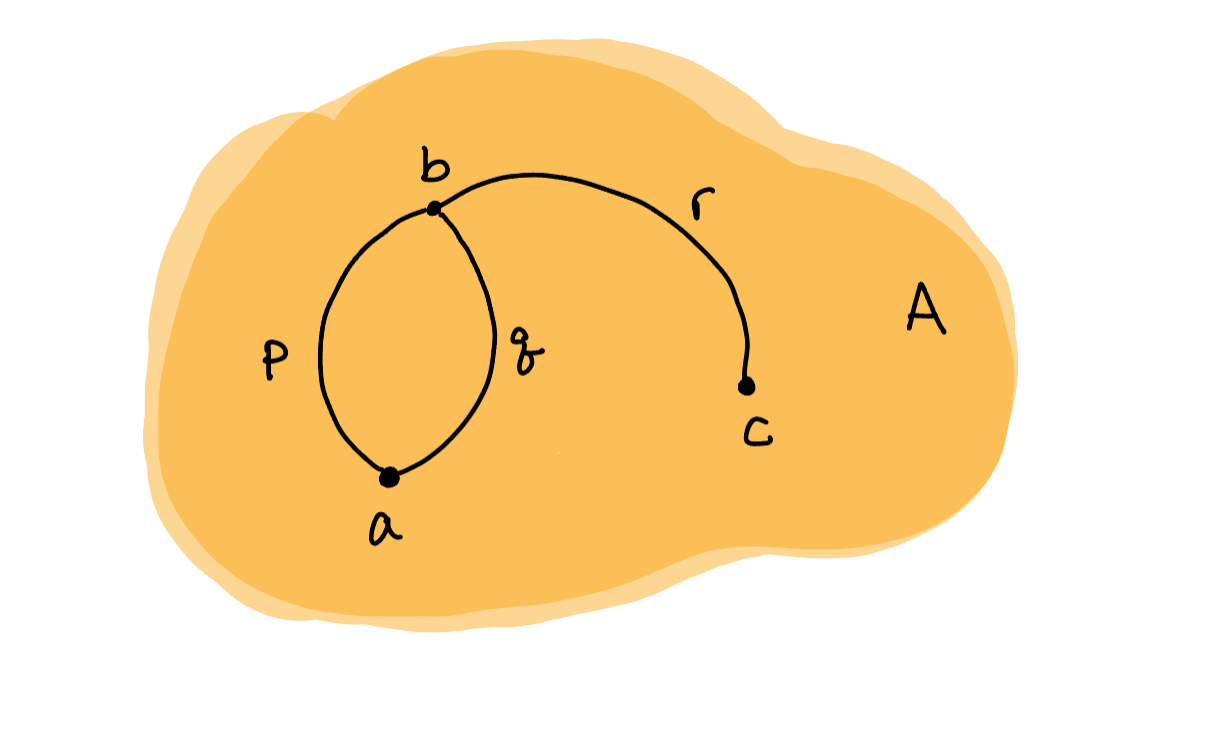
\includegraphics[scale=0.5]{disk.png}
    \caption{A disk-shaped space $A$ and points $a$, $b$, and $c$ and paths $p$, $q$, and $r$.
    The paths $p$ and $q$ can be deformed to each other without leaving the space $A$.}
    \label{fig:disk}
\end{figure}

\begin{figure}[h]
    \centering
    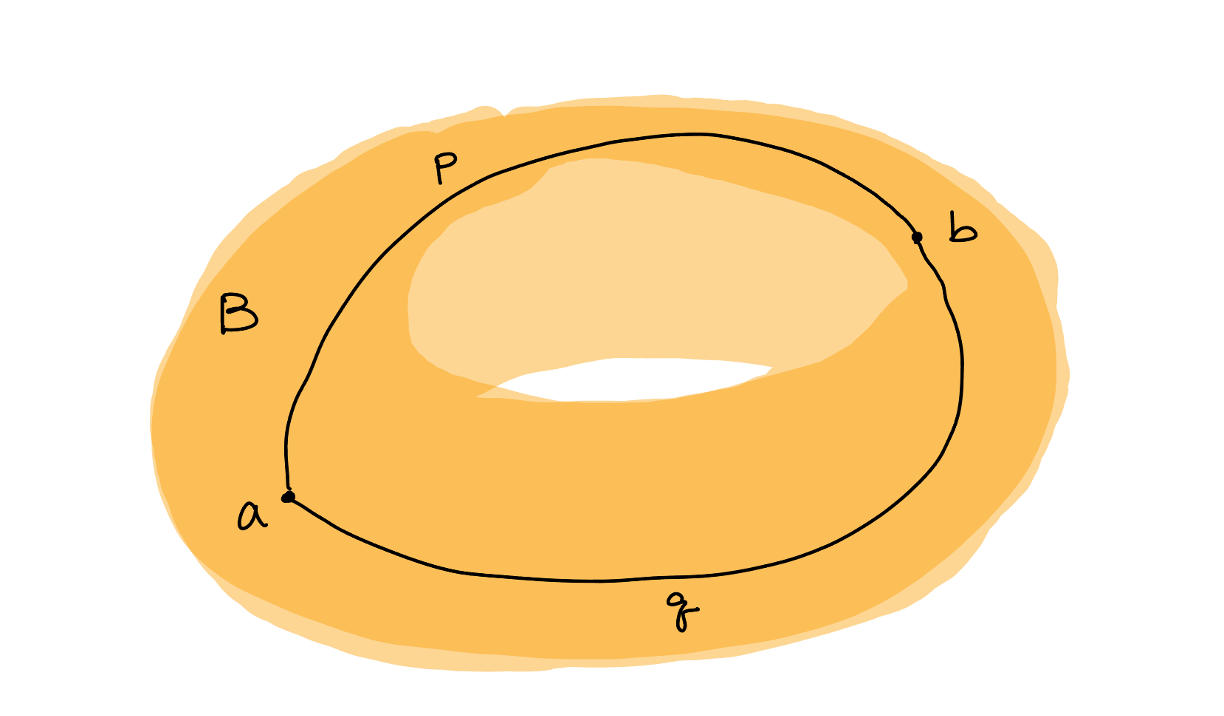
\includegraphics[scale=0.5]{torus.png}
    \caption{A torus-shaped space $B$ and points $a$ and $b$ and paths $p$ and $q$.
    The two paths can't be deformed to each other without leaving the space $B$.}
    \label{fig:torus}
\end{figure}

%Why is this "the first homotopical phenomenon"
%Make the diagram

\begin{ex}[Symmetry]\label{ex:id-symmetry}
    Define a function that produces the inverse of a path.
    \[
        (-)^{-1} : (a = b) \to (b = a)
    \]
\end{ex}

\begin{ex}[Transitivity]\label{ex:id-transitivity}
    Define a function that produces the composition of two paths.
    \[
        - \cdot - : (a = b) \to (b = c) \to (a = c)
    \]
\end{ex}

\begin{table}[h]
    \centering
    \begin{tabular}{|c|c|}\hline
        Equality & Homotopy \\\hline
        reflexivity & constant path \\\hline
        symmetry & inverse path \\\hline
        transitivity & path concatenation \\\hline
    \end{tabular}
    \caption{Exercises \ref{ex:id-symmetry} and \ref{ex:id-transitivity} reveal the connections between identity types and homotopies.}
    \label{tab:equalities-and-homotopy}
\end{table}

\begin{ex}
    Give an example of two equalities in some type that are equal to each other in the relevant identity type and prove that they are equal, i.e., pick a specific type $A$ and two terms $a$ and $b$, construct two distinct terms $p, p' : a =_A b$, and prove $\alpha : p \mathbf{=}_{a =_A b} p'$.
\end{ex}

\begin{ex}
    Show that functions $f : A \to B$ respect equalities.
    In other words, construct the following function:
    \[
        \mathsf{ap}_{f} : (a =_{A} b) \to (f(a) =_{B} f(b))
    \]
    The notation $\mathsf{ap}_{f}$ can be read as the \underline{a}ction on \underline{p}aths of $f$ \cite{hottbook}.
\end{ex}

%\begin{figure}[h]
%    \centering
%    \begin{tikzpicture}
\node at (4,0) {$B$};
\node at (5,5) {$\Sigma_{x : B}E(x)$};

\node at (-2,0) {$a$};
\draw[black,fill=black] (-1.5,0) circle (.5ex);

\node at (2.5,0) {$b$};
\draw[black,fill=black] (2,0) circle (.5ex);

\draw (0,5) ellipse (4cm and 1.3cm);
\draw (0,0) ellipse (3cm and 1cm);

\path[draw, snake it] (-1.5,0) -- (2,0);

\node at (0, 0.5) {$p$};

\node at (-2,5) {$f(a)$};
\draw[black,fill=black] (-1.5,5) circle (.5ex);

\node at (2.5,5) {$f(b)$};
\draw[black,fill=black] (2,5) circle (.5ex);

\path[draw, snake it] (-1.5,5) -- (2,5);
\node at (0, 5.5) {$\mathsf{ap}_{f}~p$};

\node at (0.4,2.2) {$\pi_{1}$};
\draw[->] (0,3) -- (0,1.5);
\end{tikzpicture}
%    \caption{Caption}
%    \label{fig:ap}
%\end{figure}

Veovosky showed that MLTT can be interpreted in a category of spaces (the category of Kan complexes).
\begin{table}[h]
    \centering
    \begin{tabular}{|c|c|}\hline
        MLTT & Space\\\hline
        types $T$ & spaces $T$\\\hline
        terms $t$ & points $t \in T$\\\hline
        dependent types $x : B \vdash E(x) \type$ & fibrations 
            $\begin{array}{c}
            E\\
            \downarrow\\
            B
            \end{array}$\\\hline
        equalities & paths/homotopies\\\hline
    \end{tabular}
    \caption{The space interpretation of MLTT.}
    \label{tab:the-space-interpretation-of-mltt}
\end{table}

\begin{ex}[Transport]
    Show that for any dependent type $x : B \vdash E(x) \type $, any terms $b, b' : B$, and any path $p : b =_B b'$, there is a function $p_{*} : E(b) \to E(b')$.
\end{ex}
This ensures that every dependent type we can construct respects propositional equality. 
If we think of $E$ as a predicate on $B$, this means that if $E(b)$ is true and $b =_B b'$, then $E(b')$ is true.

This is part of a more sophisticated relationship between type theory and homotopy theory (Quillen model category theory, or QMC theory). 
Transport says that $\pi_{1} : \Sigma_{b : B} E(b) \rightarrow B$ behaves like a fibration in a QMC. For more information, see Appendix $\ref{sec:transport-explanation}$.

\section{Characterizing Equality in Standard Types}

\begin{itemize}
\item[\Bool:] We can show $\False = \False$,
$\True = \True$,
$\False \neq \True$. (Note that $\False \neq \True$ means that there is a function $\False \neq \True$ defined as $(\False = \True)\to \emptyset$. More generally, $\neg P$ is defined as $P\to\emptyset$.)
\item[$\N$:] We can show $S n = S m \Rightarrow n = m$ and $0 \neq S n$.
\item[$\Sigma$-types:] We can show that for all $s, t : \Sigma_{a : A} B(a)$, we have $(s \mathbf{=}_{\Sigma_{a : A} B(a)} t) \simeq \Sigma_{p : \pi_1 s = \pi_1 t} \mathbf{tr}_p \pi_2 s = \pi_2 t$.
\item[$\Pi$-types:] \textsc{(functional extensionality)} We might want that $\forall f, g : \Pi_{a : A} B(a)$, $(f = g) \simeq \Pi_{x : A} f(x) = g(x)$, but this is functional extensionality ($\mathbf{funext}$), and it is \textbf{not provable} in MLTT. This is validated by interpretations  in logic, sets, and spaces (i.e., functional extentionality is true in all of those systems).
\item[$=$-types:] \textsc{(uniqueness of identity proofs)} We might want that $\forall p, q : a = b$, $(p = q) \simeq \mathbbm{1}$, but this is uniqueness of identity proofs (UIP), which is \textbf{not provable} in MLTT. This is validated by interpretations in logic and sets, but not in spaces. 
\item[$U$-types:] \textsc{(univalence)} We might want that $\forall S, T : U$, $(S = T) \simeq (S \simeq T)$, but this is univalence ($\mathbf{UA}$), which is \textbf{not provable} in MLTT. This is validated by interpretation in \textbf{spaces}.
\end{itemize}

\begin{figure}[h]
    \centering
    % https://q.uiver.app/#q=WzAsMyxbMCwwLCJVQSJdLFs2LDAsIlVJUCArIEVSIl0sWzMsMywiRnVuRXh0Il0sWzAsMiwiaW1wbGllcyIsMl0sWzEsMiwiaW1wbGllcyJdLFswLDEsImluY29tcGF0aWJsZSIsMCx7InN0eWxlIjp7ImJvZHkiOnsibmFtZSI6InNxdWlnZ2x5In0sImhlYWQiOnsibmFtZSI6Im5vbmUifX19XV0=
\[\begin{tikzcd}
	\mathrm{UA} &&&&&& {\mathrm{UIP \& ER}} \\
	\\
	\\
	&&& \mathrm{FunExt}
	\arrow["\mathrm{Implies}"', from=1-1, to=4-4]
	\arrow["\mathrm{Implies}", from=1-7, to=4-4]
	\arrow["\mathrm{Incompatible}", squiggly, no head, from=1-1, to=1-7]
\end{tikzcd}\]
    \caption{Both UA and UIP with equality reflection (ER) imply functional extensionality.
    However, UA and UIP are incompatible.}
    \label{fig:ua-uip-funext}
\end{figure}

To avoid inconsistency, we cannot have both $\mathbf{UA}$ and $\mathbf{UIP}$. We choose $\mathbf{UA}$ (and so also get $\mathbf{funext}$). 
Both choices make sense, but choosing $\mathbf{UIP}$ would send us in the direction of set theory, not HoTT.

\section{Homotopy Levels}
Types in HoTT come equipped with higher-dimensional structures.
In some types, however, these structures are trivial above a certain dimension.
In this section, we introduce \emph{homotopy levels}, or h-levels for short, and discuss some special cases.

\subsection{h-level 0}\label{sec:h-level-0}
A type $T$ is \emph{contractible} (has h-level 0) if there is a \emph{center of contraction} $t$, and for every inhabitant $s$ of that type there is a path from $s$ to $t$.
\[
    \isContr(T) := \sum_{t : T}\prod_{s : T} (s = t)
\]
\begin{figure}[h]
    \centering
    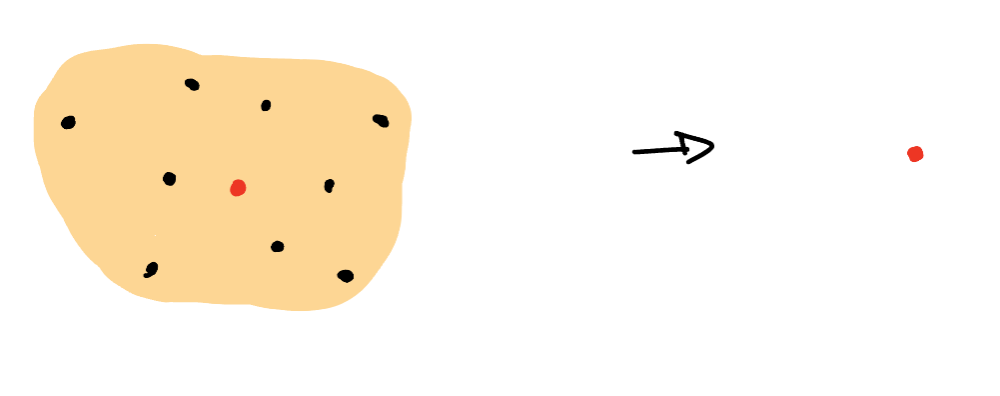
\includegraphics[scale=0.5]{hlvl0.png}
    \caption{A type $T$ with h-level 0 has a center of contraction $t$ and every inhabitant has a path to $t$.}
    \label{fig:h-level-0}
\end{figure}

For example, the unit type $\Unit$ is contractible.
Choose $\mathsf{tt}$ to be the center of contraction.
The result follows by the elimination rule for $\Unit$.

\begin{ex}
Show that if $T$ is contractible and inhabited, then $T \simeq \mathbbm{1}$.
\end{ex}

%\begin{figure}[h]
%    \centering
%    \begin{tikzpicture}
    \draw (0,0) circle (3cm);
    \node (t) at (0,0) {};
    \draw[black, fill=black] (0, 0) circle (.5ex);

    \node (1) at (2,2) {};
    \node (2) at (-1.3,1) {};
    \node (3) at (-2.3,-0.3) {};
    \node (4) at (1.7,-2);

    \draw[->] (1) -- (t);
    \draw[->] (2) -- (t);
    \draw[->] (3) -- (t);
    \draw[->] (4) -- (t);
\end{tikzpicture}
%    \caption{Caption}
%    \label{fig:h-level0}
%\end{figure}

\subsection{h-level 1}\label{sec:h-level-1}
A type $T$ is a \emph{proposition} (has h-level 1) if for any $s, t : T$ the identity type $s = t$ is contractible.
\[
    \isProp(T) := \prod_{s,t : T}\isContr(s = t)
\]
Note that a proposition does not need to be inhabited.
For example, the empty type $\varnothing$ is a proposition.
See Exercise \ref{ex:empty-unit-prop}.
\begin{figure}[h]
    \centering
    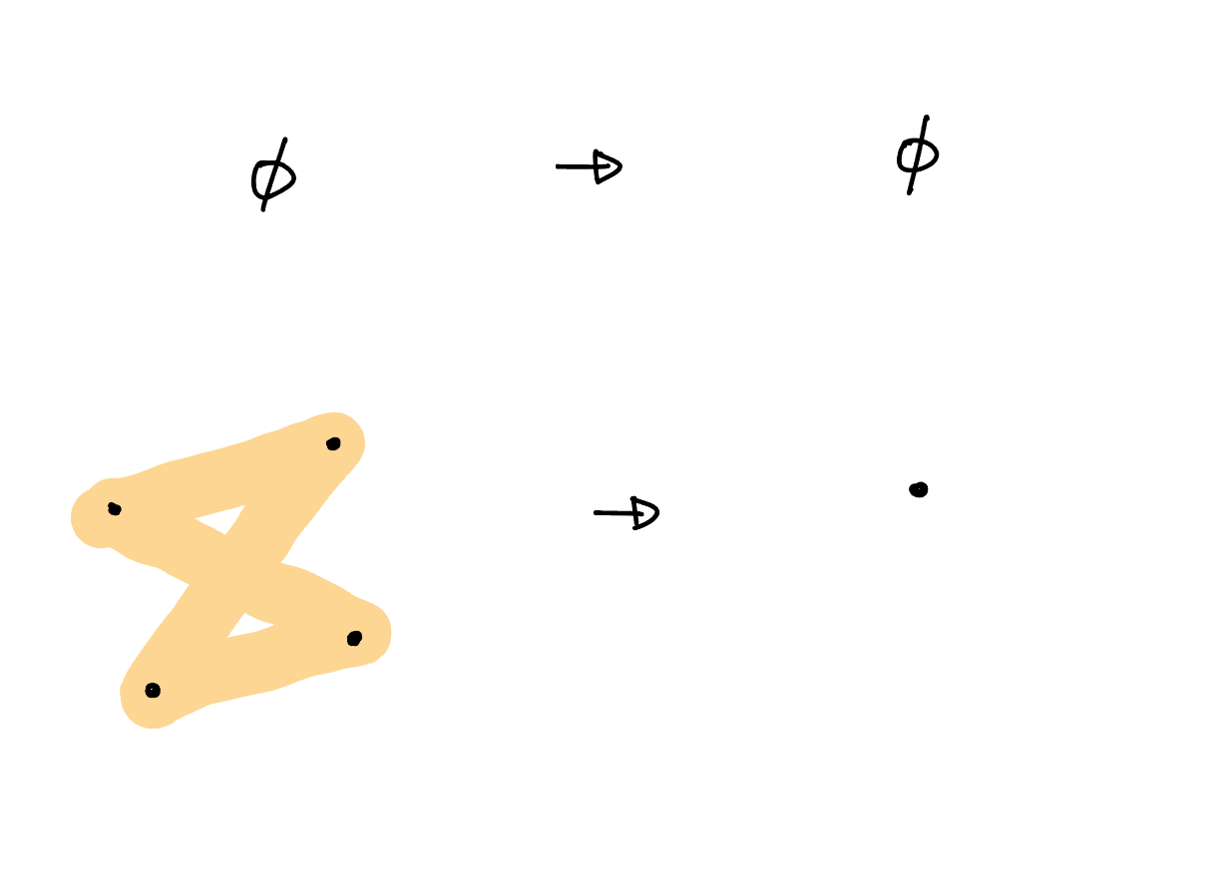
\includegraphics[scale=0.5]{hlvl1.png}
    \caption{If a type $T$ has h-level 1, then the identity type $s = t$ between any two inhabitants $s$ and $t$ is contractible.
    This means that any two proofs of a proposition are equal.}
    \label{fig:h-level-1}
\end{figure}

\begin{ex}\label{ex:empty-unit-prop}
Show that $\emptyset$, $\mathbbm{1}$ are propositions.
\end{ex}

\begin{ex}
Show that any contractible type is a proposition.
\end{ex}

\begin{ex}
Show that if a proposition is inhabited, then it is contractible. (This says that a proposition is informally equivalent to $\varnothing$ or $\mathbbm{1}$, i.e., truth values) %I don't think this is actually what this exercise shows but I'm not sure what the correct interpretation of this comment in the notes is
\end{ex}

\subsection{h-level 2}\label{sec:h-level-2}
A type $T$ is a \emph{set} (has h-level 2) if for any $s, t : T$ the identity type $s = t$ is a proposition.
\[
    \isSet(T) := \prod_{s,t : T}\isProp(s = t)
\]
In other words, $T$ is a set if it looks like a discrete collection of points.
For example, the types $\N$ and $\Bool$ are sets.
\begin{figure}[h]
    \centering
    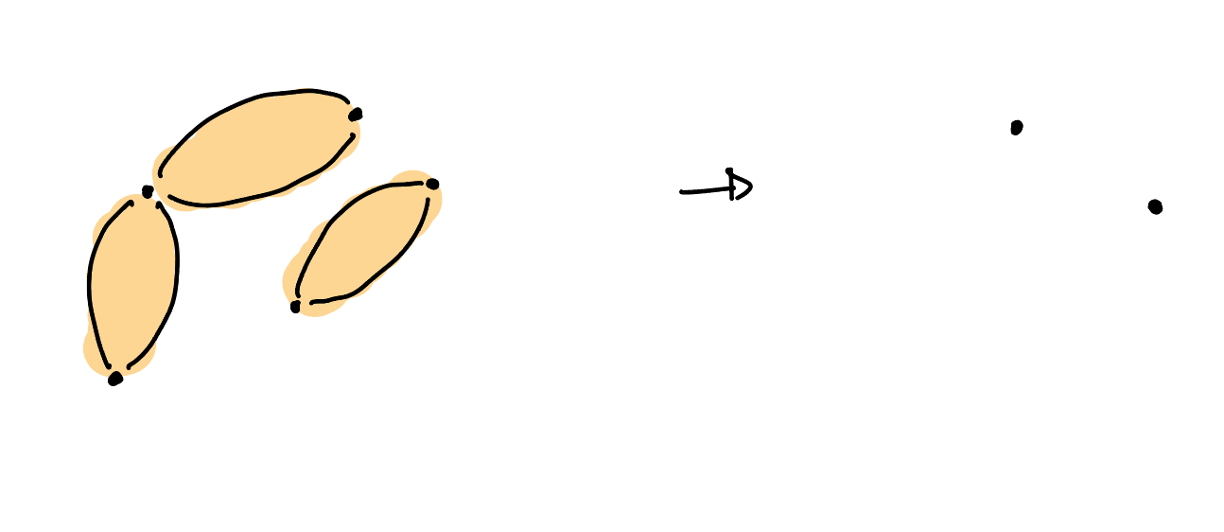
\includegraphics[scale=0.5]{hlvl2.png}
    \caption{If a type $T$ has h-level 2, then the identity type $s = t$ between any two inhabitants $s$ and $t$ is a proposition.
    Thus, $T$ looks like a set.}
    \label{fig:h-level-2}
\end{figure}

\subsection{h-level 3}\label{sec:h-level-3}
A type $T$ is a \emph{groupoid} (has h-level 3) if for any $s, t : T$ the identity type $s = t$ is a set.
\[
    \isGroupoid(T) := \prod_{s, t : T}\isSet(s = t)
\]
\begin{figure}[h]
    \centering
    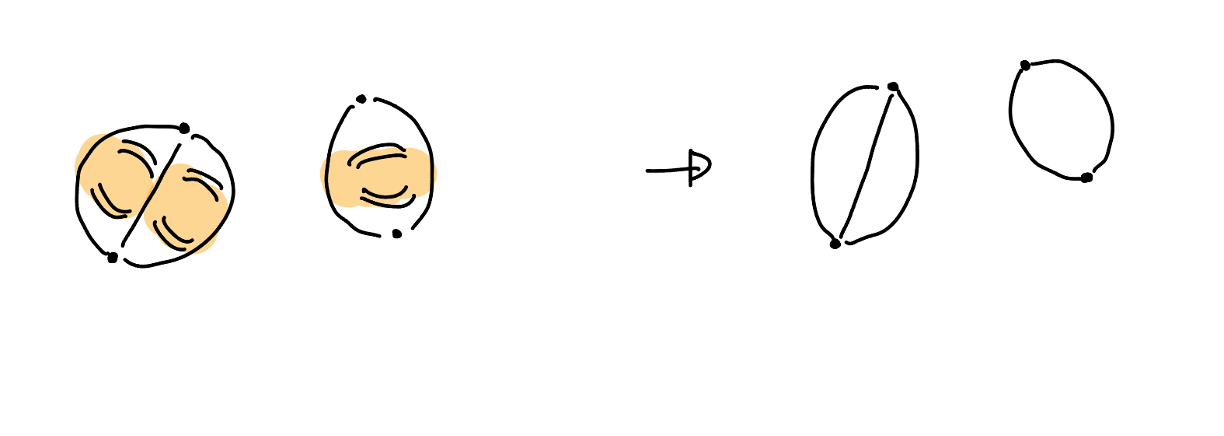
\includegraphics[scale=0.5]{hlvl3.png}
    \caption{If a type $T$ has h-level 3, then the identity type $s = t$ between any two inhabitants $s$ and $t$ is a set.
    Thus, $T$ looks like a groupoid.}
    \label{fig:h-level-3}
\end{figure}

In general, $\isofhlevel{n}{T}$ is defined recursively as follows:
\begin{align*}
    \isofhlevel{0}{T} &:= \isContr(T)\\
    \isofhlevel{S(n)}{T} &:= \prod_{s,t : T}\isofhlevel{n}{T}
\end{align*}

\begin{ex}
Show that if a type $T$ has h-level $n$, then it has h-level $n + 1$.
\end{ex}

\section{Equivalences}
Given a function $f : A \to B$, we can define $\isEquiv(f)$ by
\[
    \sum_{g : B \to A} (g \circ f = 1_{A}) \times (f \circ g = 1_{B})
\]
Sadly, this type is not a proposition.
Thus, it has nontrivial high-dimensional structures that we don't want.
To remedy this, recall that a set-theoretic function $f : A \to B$ is a bijection if for all $b \in B$, the fiber over $b$ is a singleton set.
This suggests an alternative definition for $\isEquiv(f)$.
\begin{defn}
\begin{align*}
    \isEquiv(f) &:= \prod_{b : B} \isContr\left(\sum_{a : A} f(a)=b\right)
\end{align*}
\end{defn}
This states that for every $b : B$, the fiber over $b$ is contractible, i.e., there exists a unique element in the preimage of $f$.

\begin{defn}[Equivalence]
    Given any two types $A, B : \U$, we write $A \simeq B$ to denote the type $\displaystyle\sum_{f : A \to B} \isEquiv(f)$.
\end{defn}
For any two types $A, B : \U$, we can construct a function $\idToEquiv : (A = B) \to (A \simeq B)$ by path induction.
\begin{defn}[Univalence Axiom]
    The \emph{univalence axiom} asserts that 
    \[\ua : \isEquiv(\idToEquiv)\]
\end{defn}
An immediate consequence of this axiom is that $(A = B) \simeq (A \simeq B)$.

\section{Univalence for Logic and Sets}
\begin{defn}
    We define the type of propositions as the following sigma type:
    \[\Prop := \sum_{P : \U} \isProp(P)\]
\end{defn}
The univalence axiom implies that the type $\Prop$ is univalent.
That is, for any $P, Q : \Prop$,
\[
    (P = Q) \simeq (P \leftrightarrow Q)
\]
As a corollary, the type $\Prop$ is a set rather than a proposition because there are propositions that are not interprovable, but all the interprovable ones can be identified.
We define the type of sets in the same fashion.
\begin{defn}
\[
    \Set := \sum_{S : \U} \isSet(S)
\]
\end{defn}
Similarly, the univalence axiom implies that $\Set$ is univalent.
\[
    (S = T) \simeq (S \cong T)
\]
As a consequence, $\Set$ is a groupoid because, for example, the set containing two elements is isomorphic to itself in two different ways.

With $\Set$ in hand, we can define the type of groups.
Recall that a group consists of a carrier set $G$, a neutral element $e$, a multiplication operator $\cdot$, and an inverse operator $-^{-1}$ such that
\begin{enumerate}
    \item $e \cdot g = g$ for all $g \in G$,
    \item $g \cdot e = g$ for all $g \in G$,
    \item $(g \cdot h) \cdot k = g \cdot (h \cdot k)$ for all $g, h, k \in G$,
    \item $g^{-1} \cdot g = e$ for all $g \in G$, and
    \item $g \cdot g^{-1} = e$ for all $g \in G$.
\end{enumerate}
\begin{defn}
    \begin{align*}
        \Grp := \sum_{G : \Set}&\sum_{e : G}\sum_{\cdot : G \to G \to G}\sum_{-^{-1} : G \to G}\left(\prod_{g : G} e \cdot g = g\right) \times\\
        &\left(\prod_{g : G} g \cdot e = g\right) \times \left(\prod_{g,h,k : G}(g \cdot h) \cdot k = g \cdot (h \cdot k)\right) \times\\
        &\left(\prod_{g : G}g^{-1} \cdot g = e\right) \times \left(\prod_{g : G}g \cdot g^{-1} = e\right)
    \end{align*}
\end{defn}
The role of the inhabitants of the group axioms is to serve as a \emph{witness} that the neutral element, the multiplication, and the inverse of a group interact properly.
We don't want the group axioms to carry additional structures.
Thus, the carrier $G$ needs to be a set to ensure that the group axioms are propositions.

%This encodes the existence of an identity ($e$), a partial binary operator ($m$), and an inverse operator $i$ satisfying the groupoid axioms ($e$ acts as an identity, $m$ is associative, and %inverses act as inverses). %is m partial? this seems like it's actually a group not a groupoid?

Again, the univalence axiom implies that for any two groups, $G$ and $H$,
\[(G = H)\simeq (G \cong H).\]
Similarly, we can define the type of groupoids by
\[\Grpd:= \sum_{T:\U} \isGroupoid(T)\]
In fact, any algebraic structure on a set has a univalence result \cite{coq:isomorphism-is-equality}.

%\textsc{Definition.} An algebraic structure is %needs definition from github once paige adds it there

The moral of the story is that univalence allows us to do mathematics up to some appropriate notion of ``sameness".
For example, the appropriate notion of sameness for groups is group isomorphisms.
The \textbf{Structure Identity Principle}, or \textbf{SIP} (Aczel, Coqand), is the idea that an isomorphism (or our notions of equivalence) should respect the structure of a given type.
The \textbf{Identity of Indiscernables} (Leibniz) states that any two objects that have all their properties in common cannot be distinct.
Univalence allows us to treat isomorphic, or structurally identical, types as exactly equal, incorporating these principles into our theory.

\section{Higher Inductive Types}
An ordinary inductive type, such as $\Bool$, is freely generated by its canonical terms $\True$ and $\False$.
Since we now consider types as having terms, equalities, equalities between equalities, etc, we can consider \emph{higher inductive types} whose constructors can be terms, equalities, equalities between equalities, etc.
For example, we can define the type $D^{1}$ to be generated by two points $\bullet$ and $\star$, and a path between them $p : \bullet = \star$.
The topological intuition here is that we connect the points $\bullet$ and $\star$ by adding the path $p$. 
(Here, $S^0$ stands for the $0$-dimensional sphere, and $D^1$ stands for the $1$-dimensional disc.)

\begin{itemize}
\item Formation rule: 


\begin{mathpar}
\inferrule*[right=$D^1$-Form]{ }{\Gamma \vdash D^1 \type}
\end{mathpar}

\item Introduction rules:

\begin{mathpar}
\inferrule*[right=$D^1$-Intro]{ }
{\Gamma \vdash \bullet : D^1\\\\
 \Gamma \vdash \star : D^{1}\\\\
}

\and

\inferrule*[right=$D^{1}$-Intro]{ }
{\Gamma \vdash p : \bullet = \star}
\end{mathpar}

\item Elimination rule:

\begin{mathpar}
\inferrule*[right=$D^1$-Elim]{\Gamma, x : D^1 \vdash E(x) \type \\\\
\Gamma \vdash t : E(\bullet) \\\\
\Gamma \vdash f : E(\star) \\\\
\Gamma \vdash \pi : tr(t) =_{E(\star)} f}{\Gamma, x : D^1 \vdash \Ind_{D^1, t, f, \pi} (x) : D^1(x)}
\end{mathpar}

\item Computation rules:

\begin{mathpar}
\inferrule*[right=$D^1$-Comp-T]{\Gamma, x : D^1 \vdash E(x) \type \\\\
\Gamma \vdash t : E(\bullet) \\\\
\Gamma \vdash f : E(\star) \\\\
\Gamma \vdash \pi : tr(t) =_{E(\star)} f}{\Gamma \vdash t \defeq \Ind_{D^1}(\bullet) : E(\bullet)}
\end{mathpar}

\begin{mathpar}
\inferrule*[right=$D^1$-Comp-F]{\Gamma, x : D^1 \vdash E(x) \type \\\\
\Gamma \vdash t : E(\bullet) \\\\
\Gamma \vdash f : E(\star) \\\\
\Gamma \vdash \pi : tr(t) =_{E(\star)} f}{\Gamma \vdash f \defeq \Ind_{D^1}(\star) : E(\star)}
\end{mathpar}

\begin{mathpar}
\inferrule*[right=$D^1$-Comp-$\pi$]{\Gamma, x : D^1 \vdash E(x) \type \\\\
\Gamma \vdash t : E(\bullet) \\\\
\Gamma \vdash f : E(\star) \\\\
\Gamma \vdash \pi : tr(t) =_{E(\star)} f}{\Gamma \vdash \Ind_{D^1}(p) = \pi : tr(t) = f}
\end{mathpar}

\end{itemize}

Similarly we can define $S^1$ as being generated by $b : S^1$ and $l : b \mathbf{=}_{S^1} b$ ($b$ can be thought of as a base point and $l$ can be thought of as a loop).

We have the following classical result about the fundamental group of the circle:
\begin{fact}
$\pi_1(S^1)\simeq \Z$.
%    $\pi_1 (\Sigma_{S^1 : U} S^1) \simeq \mathbbm{Z}$, where $\pi_1 (\Sigma_{T : U} T)$ is a function from $\Sigma_{S^1 : U} S^1$ to $\Sigma_{T : U} T$ taking $b$ to the witness for $T$. $\pi_1$ is thus a way to make an arbitrary type into a Set.
\end{fact}
In the fact above, $\pi_1(T,t) := (S^1,b) \to (T,t)$, where the right-hand side stands for the function from $S^1$ to $T$ that sends $b$ to $t$. The pair $(T,t)$ is to be thought of as an inhabitant of the type $\Sigma_{T:\U} T$. 

\begin{defn}
    Given a type $T$, \emph{propositional truncation} $\| T \|_1$ of $T$ is the higher inductive type given by $\vert \cdot \vert_1 : T \rightarrow \| T \|_1$ and $\Pi_{x,y : T} \vert x \vert_1 = \vert y \vert_1$. 
\end{defn}

\begin{ex}
    Show that for all $T$, $\isProp(\| T \|_1)$.
\end{ex}

\begin{defn}
    Given a type $T$, the \emph{set truncation} $\| T \|_2$ of $T$ is given by $\vert \cdot \vert_2 : T \rightarrow \| T \|_2$ and $\Pi_{x : T,y : T, p : x = y, q : x = y} \vert p \vert_2 = \vert q \vert_2$.
\end{defn}

\begin{ex}
    (Optional) Show that for all $T$, $\isSet(\| T \|_2)$.
\end{ex}


\section{Category Theory}

Traditionally, a category $\cat{C}$ consists of
\begin{enumerate}
    \item a set $\ob{C}$ of objects,
    \item a set $\cHom{X}{Y}$ of morphisms for all $X, Y \in \ob{C}$,
    \item an identity morphism $\cId_{X} \in \cHom{X}{X}$ for all $X \in \ob{C}$,
    \item a composition function $\circ : \cHom{Y}{Z} \to \cHom{X}{Y} \to \cHom{X}{Z}$ for all $X, Y, Z \in \ob{C}$.
\end{enumerate}
These data are subject to the identity and associativity laws.

We could talk about categories in the set level (like most classical mathematics).
However, the structural identity principle for structures on sets tells us that 
\[(\cat{C} =_{\Cat} \cat{D}) \simeq (\cat{C} \cong \cat{D}).\]
But isomorphism is not the right kind of sameness for categories; they are too restrictive.
Instead of squashing everything down to the level of sets, HoTT affords us higher dimensional structures.

Observe that every category has a ``core groupoid" contained within it: the objects and all isomorphisms.
With a groupoid of objects in hand, we can then glue additional morphisms to this groupoid, forming a category.
\begin{defn}
    A \emph{univalent category} (or just category) $\cat{C}$ consists of:
\begin{itemize}
    \item a groupoid of objects $\ob{C} : \Grpd$;
    \item a set $\cHom{X}{Y}$ for every pair $X,Y : \ob{C}$, i.e., $$X,Y : \ob{C} \vdash \cHom{X}{Y} : \Set;$$
    \item a term $\cId_{X} : \cHom{X}{X}$ for every $X : \ob{C}$, i.e., $$X:\ob{C} \vdash \cId_{X} : \cHom{X}{X};$$
    \item a function $\circ: \cHom{Y}{Z} \to \cHom{X}{Y} \to \cHom{X}{Z}$ for every $X,Y,Z : \ob{C}$, i.e., $$X,Y,Z: \ob{C} \vdash \circ : \cHom{X}{Y} \to \cHom{Y}{Z}\to \cHom{X}{Z}$$
\end{itemize}
These data are subject to the usual axioms of categories and that the function
\[
    \idToIso: (X=Y) \to \Iso(X,Y)
\]
is an equivalence, where 
$$\Iso(X,Y) := \sum_{f:\cHom{X}{Y}} \sum_{g:\cHom{Y}{X}} (g\circ f = \cId_{X}) \times (f \circ g = \cId_{Y}).$$
Thus, the right notion of sameness for objects is isomorphism.
This additional requirement is often called (internal) univalence.
\end{defn}
The type of categories $\Cat$ can then be defined as an iterated sigma type.
Note that this is often called a \emph{univalent category} and the requirement that $\idToIso$ be an equivalence is called (internal) univalence.
As a consequence of the univalence axiom,
\[
    (\cat{C} =_{\Cat} \cat{D}) \simeq (\cat{C} \simeq \cat{D}).
\]
Thus, the terms of $\Cat$ are categories and the equalities are equivalence of categories.
\begin{cor}
    $\Cat$ is a $2$-groupoid (h-level $4$).
\end{cor}
This is a great achievement for univalent foundations.
Category theorists call definitions that are not invariant under equivalence of categories \emph{evil}.
This definition helps us avoid ``evilness" when we talk about categories.

We now define functors and natural transformations. 
\begin{defn}
    A \emph{functor} $F: \cat{C}\to\cat{D}$ consists of:
\begin{itemize}
    \item a function $\ob{F}: \ob{C}\to \ob{D}$;
    \item functions $\hom_{\mathbf C}(X,Y)\to \hom_{\mathbf D}(FX,FY)$ for all $X,Y\in \mathbf C$
\end{itemize}
such that the compositions and identities are preserved.
\end{defn}



The type of functors $[\mathcal C, \mathcal D]$ is not a set.
\begin{enumerate}
    \item terms $\rightsquigarrow$ functions;
    \item equalities $\rightsquigarrow$ natural transformations.
\end{enumerate}

\begin{defn}
    A \emph{natural transformation} $\eta: F \implies G: \mathbf{C}\to\mathbf{D}$ consists of $\eta_X:\hom(FX,GX)$ for all $X:\ob{C}$ such that the following square commutes for all $X,Y:\ob{C}$ and all $f:\hom(X,Y)$:

\begin{center}
\begin{tikzcd}
FX \arrow[r, "Ff"] \arrow[d, "\eta_X"]
& FY \arrow[d, "\eta_Y"] \\
GX \arrow[r, "Gf"]
& || GY
\end{tikzcd}
\end{center}
\end{defn}

The type of natural transformations $F\implies G$ is a set.

We can also form a \emph{bicategory} of categories. We have univalence for bicategories, as well as for any higher (but finite) algebraic structure.

\section{Rezk completion}

\begin{defn}
    A \textbf{precategory} $\cat{C}$ consists of:
    \begin{itemize}
        \item a type $\ob{C}$;
        \item sets $\hom (X,Y)$ for all $X,Y:\ob{C}$;
        \item $1_X : \hom(X,X) $ for all  $X : \ob{C}$;
        \item $\circ : \hom(X,Y)\times \hom(Y,Z)\to \hom(X,Z) $ for all $X, Y, Z : \ob{C}$;
        \item associativity axioms for $\circ$;
        \item identity axioms for $1_X$ for all $X : \ob{C}$.
    \end{itemize}
\end{defn}

\begin{defn}
    The \emph{Rezk completion} of a precategory $\mathcal C$ takes $\ob{\Rezk C}$ to be the higher inductive type given by:
    \begin{itemize}
        \item $i : \ob{C} \to \ob{\Rezk C}$;
        \item $j : \Iso(X,Y) \to i(X) \mathbf{=}_{\ob{\Rezk C}} i(Y)$;
        \item constructors for $\| \cdot \|_3$
    \end{itemize}
    This turns a precategory into a univalent category.
\end{defn}

\section{Quotient types}

\begin{defn}
    Given an equivalence relation $R$ on a set $S$, we can take the \emph{quotient} $S/R$ to be the higher inductive type given by:
    \begin{itemize}
        \item $i: S\to S/R$;
        \item for all $x, y : S$, the function $j_{x,y} : (xRy) \to (i(x) = i(y))$;
        \item constructors for $\| \cdot \|_2$.
    \end{itemize}
\end{defn}

\bibliographystyle{alpha}
\bibliography{all}

\appendix

\section{Transport and Fibrations}
\label{sec:transport-explanation}

As mentioned earlier, the ability to transport along an equality corresponds to the projection map $\pi_1 : \Sigma_{b : B} E(b)$ behaving like a fibration in a QMC. We will now discuss one way to see this, taking the liberty to interpret equalities as a map from the interval type into the target type, as is possible in a QMC (as well as in cubical formulations of HoTT).

\begin{figure}[h]
    \centering
    % https://q.uiver.app/#q=WzAsNCxbMCwwLCIqIl0sWzIsMCwiXFxTaWdtYV97YiA6IEJ9IEUoYikiXSxbMCwyLCJJIl0sWzIsMiwiQiJdLFsyLDMsInAiLDJdLFswLDEsIlxcdGV4dHtjb25zdH1feyhiLCBlKX0iXSxbMCwyLCJcXHRleHR7Y29uc3R9X3swfSIsMl0sWzEsMywiXFxwaV8xIl0sWzIsMSwiaCIsMix7InN0eWxlIjp7ImJvZHkiOnsibmFtZSI6ImRhc2hlZCJ9fX1dXQ==
\[\begin{tikzcd}
	{*} && {\Sigma_{b : B} E(b)} \\
	\\
	I && B
	\arrow["p"', from=3-1, to=3-3]
	\arrow["{\text{const}_{(b, e)}}", from=1-1, to=1-3]
	\arrow["{\text{const}_{0}}"', from=1-1, to=3-1]
	\arrow["{\pi_1}", from=1-3, to=3-3]
	\arrow["h"', dashed, from=3-1, to=1-3]
\end{tikzcd}\]
    \caption{Given that the outer diagram commutes, we have that if $\pi_1$ is a fibration, there exists a homotopy lifting map $h$ making everything commute.}
    \label{fig:transport-as-fibration}
\end{figure}

Consider Figure \ref{fig:transport-as-fibration}. If the outer diagram commutes, we have the data $b : B$, $e : E(b)$, and a path $p : b = b'$ for some (unstated) $b' : B$.

This follows because, when interpreting $p$ as a map from $I$ to $B$, evaluating $p$ at $0 : I$ must result in $b$ by commutativity.

Then, if $\pi_1$ is a fibration, we get that there exists a homotopy lift $h : (b, e) = (b', e')$ for some (unstated) $e' : E(b')$ that makes the diagram commute.

This is because, when interpreting $h$ as a map from $I$ to $\Sigma_{b : B} E(b)$, evaluating $p$ at $0 : I$ must result in $(b, e)$ by commutativity.

Furthermore, evaluating $h$ at $1 : I$ and then applying $\pi_1$ must result in the same value as evaluating $p$ at $1 : I$, also by commutativity.

Thus, given such an $h$, we can define $tr_p (e)$ to equal $\pi_2 (h (1)) : E(b')$. Thus, if $\pi_1$ is always a fibration, given a term $p : b = b'$, we can define $tr_p : E(b) \to E(b')$.

In the reverse direction, given a term $tr_p : E(b) \to E(b')$ along with the property that $tr_{r_b} \defeq \text{id}_{E(b)}$ (which holds when defining transport using path induction), given that the outer diagram in Figure \ref{fig:transport-as-fibration} commutes, we can define $h : (b, e) = (b', tr_p (e))$.

To do this, we can use the elimination rule for identity types to reduce this problem to the case where $b' \defeq b$ and $p \defeq r_b$. As such, we now want to define $h : (b, e) = (b', tr_{r_b} (e))$.

But as $(b', tr_{r_b} (e))$ definitionally reduces to $(b, \text{id}_{E(b)} (e))$ and then again to $(b, e)$, we get that $h : (b, e) = (b, e)$.

As such, we can just let $h$ be $r_{(b, e)}$ to finish the proof.

Thus, we have that if $\pi_1$ is a fibration, we can construct transport along a path $p : b = b'$ as $tr_b : E(b) \to E(b')$, and if we have transport we can show that $\pi_1$ is a fibration.

As a bonus exercise, prove that this map taking in $tr_p$ and output $h$ is an equivalence!

\section{Solutions}
\label{sec:exercise-solutions}
\begin{sol}[\ref{ex:not}]
    The function $\mathsf{not}$ has the following definitional equalities:
    \begin{enumerate}
        \item $\mathsf{not}~\False \defeq \True$
        \item $\mathsf{not}~\True \defeq \False$
    \end{enumerate}
    Let $b : \Bool$ be given and $b : \Bool \vdash \Bool \type$ be the motive of induction.
    By induction on $b$, it suffices to specify $\vdash \Hole{1} : \Bool$ and $\vdash \Hole{2} : \Bool$.
    \begin{mathpar}
        \inferrule*[right=Abs]
        {
            \inferrule*[Right=Bool-Elim]
            {b : \Bool \vdash \Bool \type \\ 
            \vdash \Hole{1} : \Bool \\ 
            \vdash \Hole{2} : \Bool}
            {b : \Bool \vdash \Ind_{\Bool,\Hole{1},\Hole{2}}(b) : \Bool}
        }
        {\vdash \lambda b : \Bool.~\Ind_{\Bool,\Hole{1},\Hole{2}}(b) : \Bool \to \Bool}
    \end{mathpar}
    To satisfy the first definitional equality, we choose $\Hole{1} := \True$.
    Similarly, to satisfy the second definitional equality, we choose $\Hole{2} := \False$.
    \begin{mathpar}
        \inferrule*[right=Abs]
        {
            \inferrule*[Right=Bool-Elim]
            {b : \Bool \vdash \Bool \type \\ 
            \vdash \True : \Bool \\ 
            \vdash \False : \Bool}
            {b : \Bool \vdash \Ind_{\Bool,\True,\False}(b) : \Bool}
        }
        {\vdash \lambda b : \Bool.~\Ind_{\Bool,\True,\False}(b) : \Bool \to \Bool}
    \end{mathpar}
    \begin{warn}
        The order of $\Hole{1}$ and $\Hole{2}$ is reversed in the Coq implementation.
    \end{warn}
\end{sol}

\begin{sol}[\ref{ex:iota}]
    The function $\iota$ has the following definitional equalities:
    \begin{enumerate}
        \item $\iota~\False \defeq 0$
        \item $\iota~\True \defeq 1$
    \end{enumerate}
    Let $b : \Bool$ be given and $b : \Bool \vdash \N \type$ be the motive of induction.
    By induction on $b$, it suffices to specify two terms, $\vdash \Hole{1} : \N$ and $\vdash \Hole{2} : \N$.
    \begin{mathpar}
        \inferrule*[right=Abs]
        {
            \inferrule*[Right=Bool-Elim]
            {b : \Bool \vdash \N \type \\\\ \vdash \Hole{1} : \N \\ \vdash \Hole{2} : \N}
            {b : \Bool \vdash \Ind_{\Bool,\Hole{1},\Hole{2}}(b) : \Bool}
        }
        {\vdash \lambda b : \Bool.~\Ind_{\Bool,\Hole{1},\Hole{2}}(b) : \Bool \to \N}
    \end{mathpar}
    To satisfy the definitional equalities, we choose $\Hole{1} := 0$ and $\Hole{2} := 1$.
    \begin{mathpar}
        \inferrule*[right=Abs]
        {
            \inferrule*[Right=Bool-Elim]
            {b : \Bool \vdash \N \type \\\\ \vdash 0 : \N \\ \vdash 1 : \N}
            {b : \Bool \vdash \Ind_{\Bool,0,1}(b) : \Bool}
        }
        {\vdash \lambda b : \Bool.~\Ind_{\Bool,0,1}(b) : \Bool \to \N}
    \end{mathpar}
    \begin{warn}
        The order of $\Hole{1}$ and $\Hole{2}$ is reversed in the Coq implementation.
    \end{warn}
\end{sol}

\begin{sol}[\ref{ex:add}]
    The function $\mathsf{add}$ has the following definitional equalities:
    \begin{enumerate}
        \item $\mathsf{add}~n~0 \defeq n$
        \item $\mathsf{add}~n~S(m) \defeq S(\mathsf{add}~n~m)$
    \end{enumerate}
    Let $n : \N$, $m : \N$ be given, and $n : \N, m : \N \vdash \N \type$ be the motive of induction.
    By induction on $m$, it suffices to specify $n : \N \vdash \Hole{1} : \N$ and $n : \N, m : \N, h : \N \vdash \Hole{2} : \N$.
    \begin{mathpar}
        \inferrule*[right=Abs]
        {
            \inferrule*[Right=$\N$-Elim]
            {n : \N, m : \N \vdash \N \type \\\\ 
             n : \N \vdash \Hole{1} : \N \\\\ 
             n : \N, m : \N, h : \N \vdash \Hole{2} : \N}
            {n : \N, m : \N \vdash \Ind_{\N,\Hole{1},\Hole{2}}(m) : \N}
        }
        {\vdash \lambda n : \N.~\lambda m : \N.~\Ind_{\N,\Hole{1},\Hole{2}}(m) : \N \to \N \to \N}
    \end{mathpar}
    To satisfy the first definitional equality, choose $\Hole{1} := n$.
    To satisfy the second definitional equality, choose $\Hole{2} := S(h)$
    \begin{mathpar}
        \inferrule*[right=Abs]
        {
            \inferrule*[Right=$\N$-Elim]
            {n : \N, m : \N \vdash \N \type \\\\ 
             n : \N \vdash n : \N \\\\ 
             n : \N, m : \N, h : \N \vdash S(h) : \N}
            {n : \N, m : \N \vdash \Ind_{\N,n,S(h)}(m) : \N}
        }
        {\vdash \lambda n : \N.~\lambda m : \N.~\Ind_{\N,n,S(h)}(m) : \N \to \N \to \N}
    \end{mathpar}
\end{sol}

\begin{sol}[\ref{ex:mult}]
    The function $\mathsf{mult}$ has the following definitional equalities:
    \begin{enumerate}
        \item $\mathsf{mult}~n~0 \defeq 0$
        \item $\mathsf{mult}~n~S(m) \defeq \mathsf{add}~n~(\mathsf{mult}~n~m)$
    \end{enumerate}
    Let $n : \N$, $m : \N$ be given, and $n : \N, m : \N \vdash \N \type$ be the motive of induction.
    By induction on $m$, it suffices to specify $n : \N \vdash \Hole{1} : \N$ and $n : \N, m : \N, h : \N \vdash \Hole{2} : \N$.
    \begin{mathpar}
        \inferrule*[right=Abs]
        {
            \inferrule*[Right=$\N$-Elim]
            {n : \N, m : \N \vdash \N \type \\\\ 
             n : \N \vdash \Hole{1} : \N \\\\ 
             n : \N, m : \N, h : \N \vdash \Hole{2} : \N}
            {n : \N, m : \N \vdash \Ind_{\N,\Hole{1},\Hole{2}}(m) : \N}
        }
        {\vdash \lambda n : \N.~\lambda m : \N.~\Ind_{\N,\Hole{1},\Hole{2}}(m) : \N \to \N \to \N}
    \end{mathpar}
    To satisfy the first definitional equality, choose $\Hole{1} := 0$.
    To satisfy the second definitional equality, choose $\Hole{2} := \mathsf{add}~n~h$.
    \begin{mathpar}
        \inferrule*[right=Abs]
        {
            \inferrule*[Right=$\N$-Elim]
            {n : \N, m : \N \vdash \N \type \\\\ 
             n : \N \vdash 0 : \N \\\\ 
             n : \N, m : \N, h : \N \vdash \mathsf{add}~n~h : \N}
            {n : \N, m : \N \vdash \Ind_{\N,0,\mathsf{add}~n~h}(m) : \N}
        }
        {\vdash \lambda n : \N.~\lambda m : \N.~\Ind_{\N,0,\mathsf{add}~n~h}(m) : \N \to \N \to \N}
    \end{mathpar}
\end{sol}

\section{Links and FAQ}

\begin{enumerate}
    \item \textbf{How does univalence imply functional extensionality?} Here is a blog post detailing that: \href{https://homotopytypetheory.org/2014/02/17/another-proof-that-univalence-implies-function-extensionality/}{Another proof that univalence implies functional extensionality by Dan Licata}.

    Perhaps the biggest takeaway from this article is that this proof that univalence implies functional extensionality is very closely related to the proof in cubical type theory of functional extensionality, which doesn't use univalence! There is something bigger at play here, demonstrating that univalence in some way makes things in MLTT "work better" than it used to.

    Other than that, I highly recommend checking out the article linked above, as it is by far the clearest explanation of this proof that I've seen.
    \item \textbf{Are h-levels different from universe levels?} Yes! In a type hierarchy such as the one used by Coq, each $\texttt{Type}_i$ has h-level $\infty$.
    \item \textbf{How does the inductive definition of identity types allow for non-canonical terms?} The crucial difference for identity types is that we are inductively defining a \textit{family} of types in \ref{sec:identity}. The types build by these definitions are indexed by the terms being equated, allowing us to have non-canonical terms.
\end{enumerate}

\end{document}
